\documentclass[11pt,a4paper,ngerman]{article}
\usepackage[bottom=2.5cm,top=2.5cm]{geometry} 
\usepackage{babel}
\usepackage[utf8]{inputenc} 
\usepackage[T1]{fontenc} 
\usepackage{ae} 
\usepackage{amssymb} 
\usepackage{amsmath} 
\usepackage{graphicx}
\usepackage{fancyhdr}
\usepackage{fancyref}
\usepackage{listings}
\usepackage{xcolor}
\usepackage{paralist}
\usepackage{subfigure}

%\usepackage[pdftex, bookmarks=false, pdfstartview={FitH}, linkbordercolor=white]{hyperref}
\usepackage{fancyhdr}
\pagestyle{fancy}
\fancyhead[C]{CoMa II}
\fancyhead[L]{Übung Nr. 7}
\fancyhead[R]{SoSe 2012}
\fancyfoot{}
\fancyfoot[L]{}
\fancyfoot[C]{\thepage / \pageref{LastPage}}
\renewcommand{\footrulewidth}{0.5pt}
\renewcommand{\headrulewidth}{0.5pt}
\setlength{\parindent}{0pt} 
\setlength{\headheight}{0pt}

\author{Tutor: Sebastian Scherer}
\date{}
\title{Max Wisniewski , Alexander Steen}

\begin{document}

\lstset{language=Pascal, basicstyle=\ttfamily\fontsize{10pt}{10pt}\selectfont\upshape, commentstyle=\rmfamily\itshape\small, keywordstyle=\rmfamily\bfseries, breaklines=true, frame=single, xleftmargin=3mm, xrightmargin=3mm, tabsize=2}

\maketitle
\thispagestyle{fancy}


%% ------------------------------------------------------
%%                     AUFGABE 1
%% ------------------------------------------------------

\section*{Aufgabe 1}
z.z. Alle Lösungen der DG $x' = \lambda x + f, \lambda \in \mathbb{R}$ haben die Form
$$ \alpha e^{\lambda t} + \int_0^t f(x)e^{\lambda (t-x)} \, dx  $$
für beliebiges $\alpha \in \mathbb{R}$. \\

Sei $u$ eine Lösung der Differentialgleichung, es gilt also $u'(t) = \lambda u(t) + f(t)$. Wir wollen nun zeigen, dass sich $u$ von der obigen Form nur um eine Konstante unterscheidet. Dazu bilden wir die Differenz sodass $\alpha$ auf der rechten Seite bleibt und zeigen, dass diese konstant für alle $t > 0$ ist.
Setze der Übersichtlichkeit halber $g(t) := \int_0^t f(x)e^{\lambda (t-x)} \, dx$. Dann gilt:

\begin{eqnarray*}
& & \frac{d}{dt} \left( \left( u(t) - \int_0^t f(x)e^{\lambda (t-x)} \, dx \right) e^{-\lambda t} \right)
= \frac{d}{dt} \left( (u(t) - g(t)) e^{-\lambda t} \right) \\
&=& \left( u'(t) - \frac{d}{dt} g(t) \right) e^{-\lambda t} - \lambda e^{-\lambda t} u(t) + \lambda e^{-\lambda t} g(t) \\
&=& \left( \lambda u(t) + f(t) - \frac{d}{dt} g(t) \right) e^{-\lambda t} - \lambda e^{-\lambda t} u(t) + \lambda e^{-\lambda t} g(t) \\
&=& \lambda u(t) e^{-\lambda t} + f(t)e^{-\lambda t} - \frac{d}{dt} g(t) e^{-\lambda t} - \lambda e^{-\lambda t} u(t) + \lambda e^{-\lambda t} g(t) \\
&=& f(t)e^{-\lambda t} - \frac{d}{dt} g(t) e^{-\lambda t} + \lambda e^{-\lambda t} g(t) \\
&=& e^{-\lambda t} \left( f(t) - \frac{d}{dt} g(t) + \lambda g(t) \right) \\
&=& e^{-\lambda t} \left( f(t) - g'(t) + \lambda g(t) \right) \stackrel{(*)}{=}  e^{-\lambda t} \cdot 0\\
&=& 0
\end{eqnarray*}

(*) gilt, da $g$ eine Lösung der Differentialgleichung ist (für $\alpha = 0$). \\

$ \Rightarrow \left( \left( u(t) - \int_0^t f(x)e^{\lambda (t-x)} \, dx \right) e^{-\lambda t} \right) = \alpha \in \mathbb{R}$ konstant. \\

\mbox{} \hfill $\square$
\newpage
Z.z. Die Menge aller Lösungen der DG $x' = \lambda x + f, \lambda \in \mathbb{R}$ ist ein affiner Unterraum von $V := \mathbb{R}^{[0.\infty)}$. \\


Sei $ A = \{ t \mapsto \alpha e^{\lambda t} + \int_0^t f(x)e^{\lambda (t-x)} \, dx \}$. Da für jedes $f \in A$ gilt: $f: [0,\infty) \to \mathbb{R} \Rightarrow A \subseteq V$.

Damit A ein affiner Unterraum von $V$ ist, müssen wir $A$ darstellen können als
$$ A = v + U_A $$
mit $v \in V, U_A$ Untervektorraum von $V$.

Sei $v := \int_0^t f(x)e^{\lambda (t-x)} \, dx \in V$.\\
Sei $U_A := \{ t \mapsto \alpha e^{\lambda t} | \, \alpha \in \mathbb{R} \}$.\\
z.z.: $U_A$ Untervektorraum von $V$:\\

(1) $U_A \neq \emptyset$ gilt wie man leicht sehen kann. \\
(2) $f(t), g(t) \in U_A \Rightarrow f(t)+g(t) \in U_A$. \\
Seien $f(t), g(t) \in U_A$. Dann ist $f(t) + g(t) = \alpha e^{\lambda t} + \beta e^{\lambda t} = (\alpha + \beta) e^{\lambda t} \equiv t \mapsto  (\alpha + \beta) e^{\lambda t} \in U_A$. \\
(3) $f(t) \in U_A, c \in \mathbb{R} \Rightarrow c \cdot f(t) \in U_A$. \\
Seien $f(t) \in U_A, c \in \mathbb{R}$. Dann ist $c \cdot f(t) = c \cdot \alpha e^{\lambda t} = (c \alpha)  e^{\lambda t} \equiv t \mapsto (c \alpha)  e^{\lambda t} \in U_A$.\\

$\Rightarrow U_A$ ist Untervektorraum von $V$. \\
$\Rightarrow A$ ist affiner Unteraum von $V$.
\mbox{} \hfill $\square$
%% ------------------------------------------------------
%%                     AUFGABE 2
%% ------------------------------------------------------

\section*{Aufgabe 2}
\begin{description}
\item[a)] Nach Aufgabe 1 ist die Lösung der Differentialgleichung $x'(t)  = 2x(t) + 2te^{2t}$ durch
\begin{eqnarray*}
x(t) &=& \alpha e^{2t} + \int_0^t 2xe^{2x}e^{2t-2x} \; dx\\
&=& \alpha e^{2t} + \int_0^t 2xe^{2t} \; dx\\
&=& \alpha e^{2t} + 2e^{2t} \int_0^t x \; dx\\
&=& \alpha e^{2t} + 2e^{2t} \frac{t^2}{2} \\
&=& e^{2t} (\alpha  +  t^2) \\
\end{eqnarray*}
gegeben.
Durch Einsetzen des Anfangswertes
$$
x_0 = x(0) = e^0 (\alpha + 0) = \alpha
$$
erhalten wir direkt $\alpha = x_0$ und damit
$$x(t) = e^{2t} (x_0  +  t^2)$$
als Lösung des Anfangswertproblems.

\begin{figure}[ht!]
\center
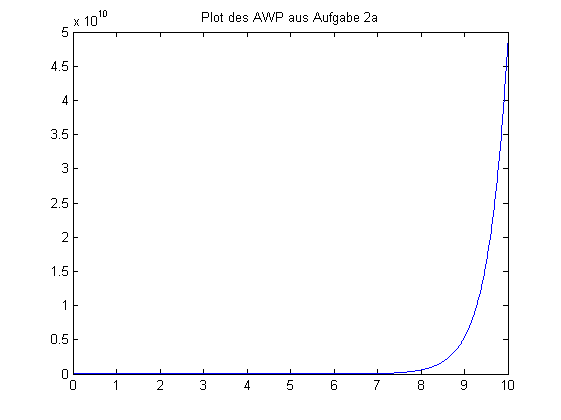
\includegraphics[scale=0.6]{ueb6auf2a.png}
\caption{Plot des AWP über dem Intervall $[0, 10]$.}
\end{figure}
\newpage
\item[b)] Für den gestörten Anfangswert erhalten wir folgenden Plot und Fehler:

\begin{figure}[ht!]
\center
\subfigure[Plot des gestörten AWP]{
	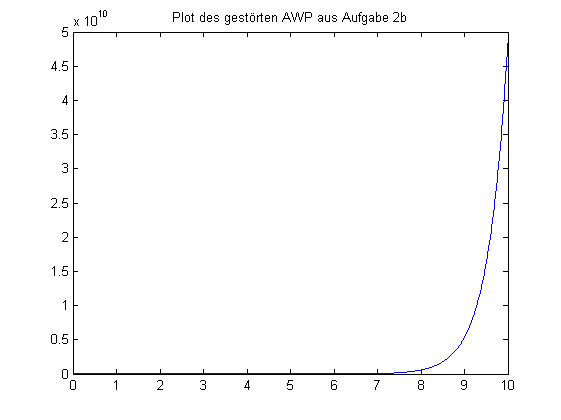
\includegraphics[scale=0.44]{ueb6auf2b.png}
}
\subfigure[Plot des Fehler $|x(t)-\tilde{x}(t)|$]{
	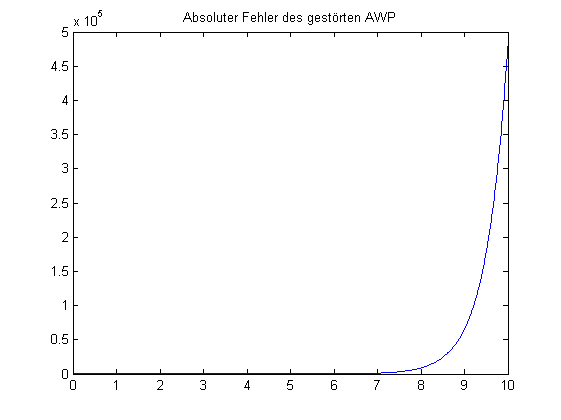
\includegraphics[scale=0.44]{ueb6auf2bfehler.png}
}
\end{figure}

\end{description}

Auffällig dabei ist, dass der absolute Fehler der beiden Plots exponentiell in $x$ steigt und bei $x = 10$ schon einen Fehler von ca. $5 \cdot 10^5$ erreicht hat. Allerdings sehen die Plots von beiden AWP sehr ähnlich aus, da sich bei einer Größenordnung von $10^10$ ein Fehler von ca. $10^5$ nicht so sehr im Plot niederschlägt. \\
Der Fehler deckt sich mit dem theoretischen Ergebnis aus der Vorlesung:\\
Hiernach ist $\| x - \tilde{x} \|_{\infty} = e^{\lambda T} |x_0 - \tilde{x}_0|$.
Bei Einsetzen von $T = 10, x_0 = 1, \tilde{x}_0 = 1.001, \lambda = 2$ erhalten wir
$$
\| x - \tilde{x} \|_{\infty} = e^{2\cdot 10} |1 - 1.001| = e^20 \cdot 0.001 \approx 4,85 \cdot 10^5
$$
als maximalen Fehler. Dies deckt sich mit dem Fehlerplot.

%% ------------------------------------------------------
%%                     AUFGABE 3
%% ------------------------------------------------------

%\section*{Aufgabe 3}


\label{LastPage}

\end{document}
